An interisting insight about the addition in propositional logic is given by the notion of \textbf{full adder}. We can think about the addition as a 
chain of operations, starting from the right-most digit. The full adder is the expression that takes in input the triple $(a_i, b_i, c_i)$ and returns the couple
($d_i, c_i$). \vspace{3.5pt}
\begin{center}
    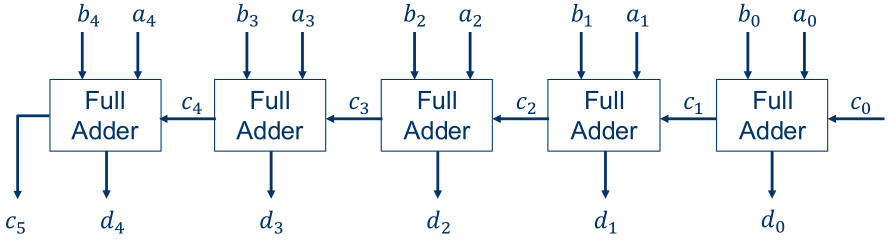
\includegraphics[width = 0.7\textwidth]{img/img36.png}
\end{center} \vspace{3.5pt}
The encoding for such chain of operations is defined as: \vspace{3.5pt}

$1^{st}$ Result $d$. \\
We can state that $d_i$ is equal to $1$ if and only if the number of ones summed up is odd, in other words:
$$d_i = a_i + b_i + c_i \ \text{mod} \ 2 \ \forall i \in \{0, \dots, n-1\}$$
The same notion can be represented as:
$$a_i \leftrightarrow b_i \leftrightarrow c_i \leftrightarrow d_i$$
that it can be expressed in CNF as:
$$d_i \leftrightarrow (a_i \wedge \neg b_i \wedge c_i) \vee (\neg a_i \wedge b_i \wedge c_i) \vee (\neg a_i \wedge \neg b_i \wedge c_i) \vee (a_i \wedge b_i \wedge c_i)$$

$2^{nd}$ Carries $c$. \\
Basically, every carry boolean variable is $1$ if and only if the sum of the triple ($a_i, b_i, c_{i-1}$) is greater than $1$.
$$c_{i+1} = 1 \leftrightarrow a_i + b_i + c_i > 1 \ \forall i \in \{0, \dots, n-1\}$$
As before, the same condition in CNF becomes:
$$c_{i+1} \leftrightarrow (a_i \wedge b_i) \vee (a_i \wedge c_i) \vee (b_i \wedge c_i)$$

$3^{rd}$ Carries $c_n$ and $c_0$. \\
Both of them must be set to $0$, in order to fit the whole sequence of bits and define the initial carry.
$$\neg c_0 \wedge \neg c_n$$